\section{Construcción del corpus}

\subsection{Extracción}
\begin{frame}
    \frametitle{Extracción}

    \begin{itemize}
        \item Humorístico: se busca en Twitter por la palabra clave \emph{chistes} y se eligen cuentas, llegando a 16.488 tweets.
        \item No humorístico: cuentas de noticias, frases filosóficas y curiosidades, alcanzando los 22.875 tweets.
    \end{itemize}
\end{frame}

\subsection{Anotación}
\begin{frame}
    \frametitle{Anotación}

    \begin{itemize}
        \item Naturalmente se etiquetarían los tweets según su tipo de cuenta; pero se encuentran muchas inconsistencias.

        \begin{itemize}
            \item Ejemplo: \emph{RT @MichelPesquera: El significado de ``Nada'' http://t.co/L1e2uHOhM4}

            \item Hay que anotarlos a mano.
        \end{itemize}

        \item Excesiva cantidad de tweets para anotar.

        \begin{itemize}
            \item Se crea una aplicación para que usuarios los anoten.
        \end{itemize}
    \end{itemize}

    \vspace{1cm}

    \begin{center}
        \bf
        Los usuarios definen al humor.
    \end{center}
\end{frame}

\begin{frame}
\frametitle{Anotación}
\framesubtitle{Cantidad de clases a considerar}
        \begin{center}
        \begin{columns}[c]
            \begin{column}[c]{0.50\textwidth}
                \centering
                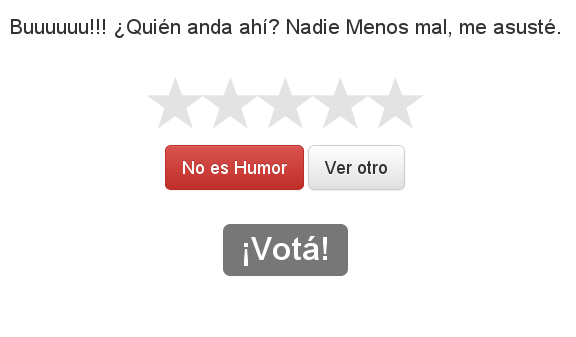
\includegraphics[frame, height=3.5cm, width=5.5cm]{pagina.png}
            \end{column}

            \begin{column}[c]{0.50\textwidth}
                \centering
                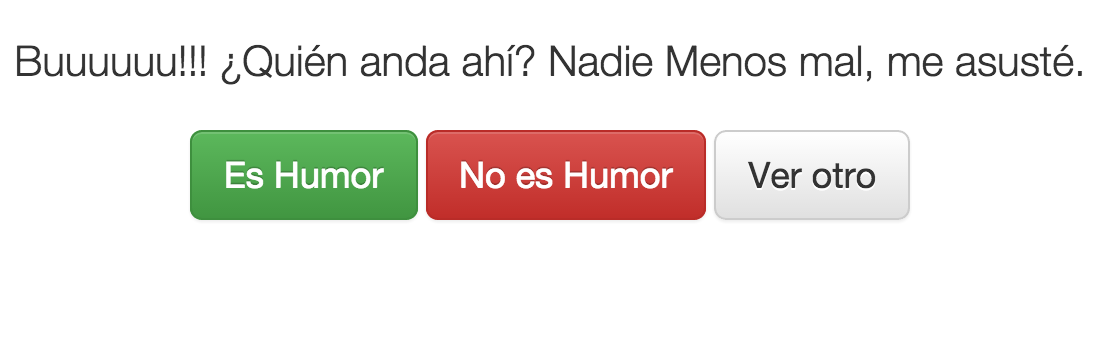
\includegraphics[frame, height=1.8cm, width=5.5cm]{pagina-dos-opciones.png}
            \end{column}
        \end{columns}
    \end{center}
\end{frame}
\begin{frame}
    \frametitle{Anotación}
    \framesubtitle{Otras consideraciones}

    \begin{itemize}
        \item Contenido explícito

        \begin{itemize}
            \item Se busca la mayor cantidad de votantes
            \item Se elimina contenido explícito
        \end{itemize}

        \item Eficiencia

        \begin{itemize}
            \item En el servidor
            \item En tiempo entre tweets
        \end{itemize}

        \item Algoritmo de selección

        \begin{itemize}
            \item Aleatorio
            \item Sin repetir
        \end{itemize}
    \end{itemize}
\end{frame}
\begin{frame}
\frametitle{Anotación}
\framesubtitle{Aplicación Final}
    \begin{center}
        \begin{columns}[c]
            \begin{column}[c]{0.45\textwidth}
                \centering
                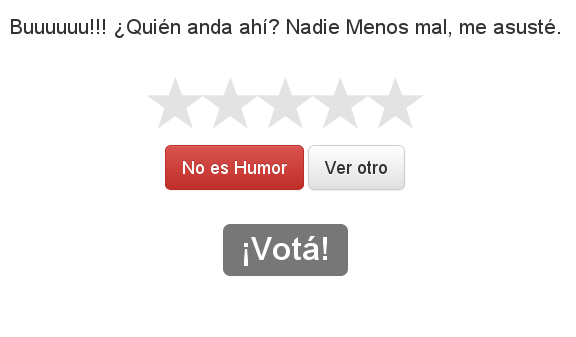
\includegraphics[frame, height=3.5cm]{pagina.png}
            \end{column}

            \begin{column}[c]{0.45\textwidth}
                \centering
                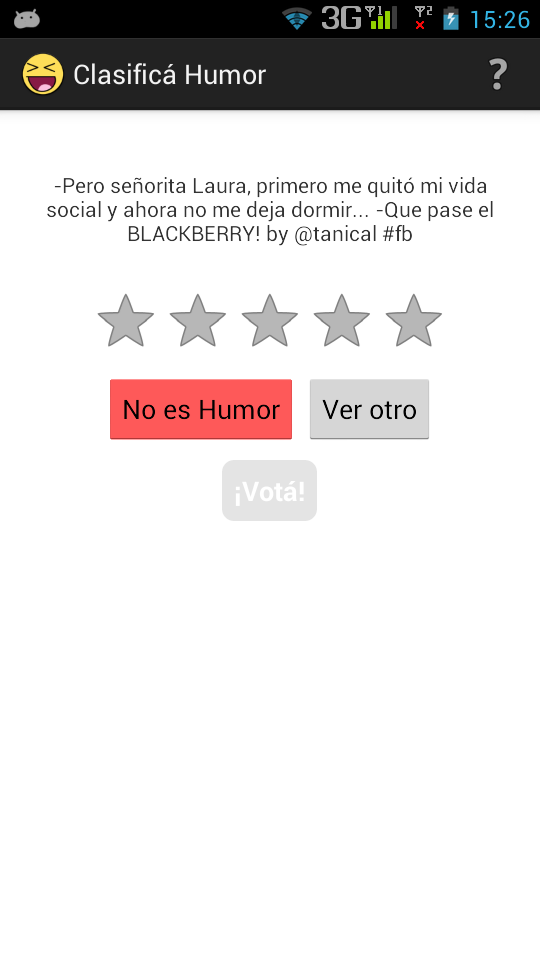
\includegraphics[frame, height=7cm]{app.png}
            \end{column}
        \end{columns}
    \end{center}
\end{frame}

\subsubsection{Resultado de la anotación}
\begin{frame}[allowframebreaks]
    \frametitle{Resultado de la anotación}

    \begin{itemize}
        \item[+] 60k votaciones recibidas
        \item[--] 20k votaciones eliminadas
        \item[--] 6,5k votaciones “ver otro” (\emph{“skip”})
        \item[=] 33,5k votos considerados
    \end{itemize}

    \framebreak

    \begin{center}
        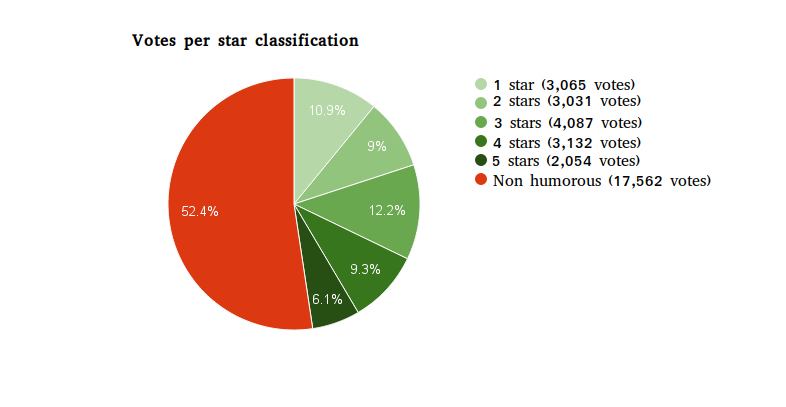
\includegraphics{votos_por_calificacion_torta.png}

        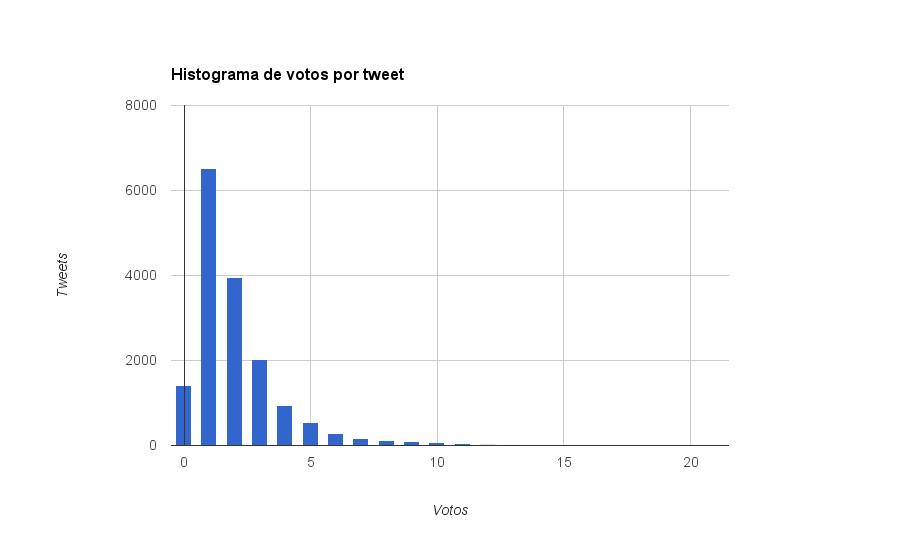
\includegraphics{histograma.png}
    \end{center}
\end{frame}

\subsubsection{Humor según la votación}

\begin{frame}[allowframebreaks]
    \frametitle{Humor según la votación}

    Porcentaje de votos positivos: $\frac{\#\{votos\ positivos\}}{\#\{total\ votos\}}$

    \begin{center}
        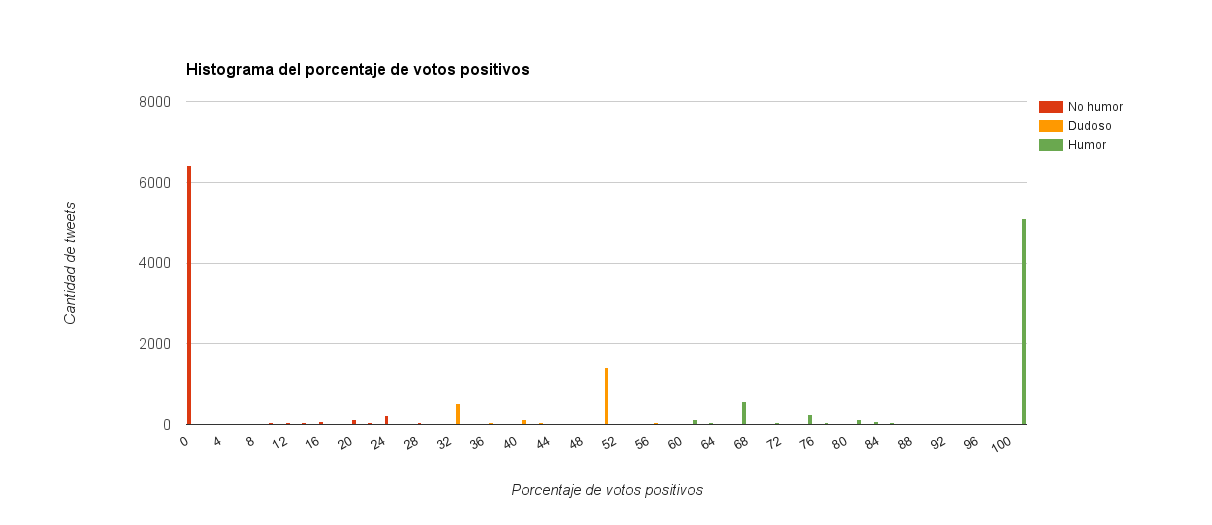
\includegraphics[height=3.75cm]{histograma_porcentaje_humor.png}
    \end{center}

    \begin{itemize}
        \item $[60\%, 100\%] \Rightarrow$ \textbf{Humor}
        \item $(30\%, 60\%) \Rightarrow$ \textbf{Dudoso}
        \item $[0\%, 30\%] \Rightarrow$ \textbf{No humor}
    \end{itemize}

    \framebreak

    \begin{center}
        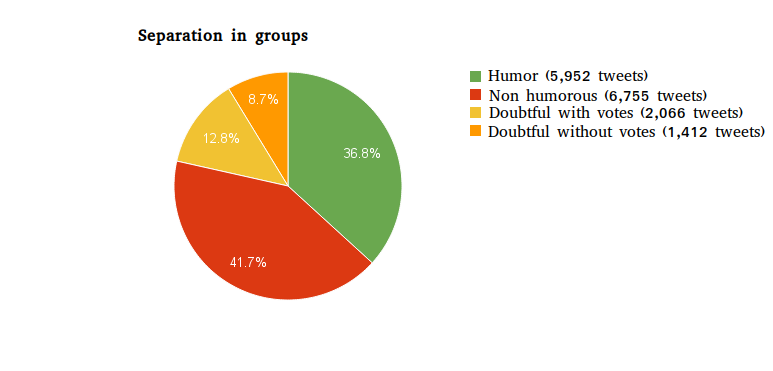
\includegraphics[height=6.5cm]{grupos.png}
    \end{center}
\end{frame}

\subsubsection{Concordancia entre los anotadores}

\begin{frame}[allowframebreaks]
    \frametitle{Concordancia entre los anotadores}

    \begin{itemize}
        \item Se quiere saber qué tan de acuerdo estuvieron las personas a la hora de votar.
        \item Se utiliza la medida kappa de Fleiss.
        \item kappa evalúa cuán mejor es la votación respecto a una al azar, siendo lo mejor posible 1 y siendo 0 una votación al azar.
    \end{itemize}

    \note{Interesa saber cuál fue la concordancia entre los anotadores, es decir, qué tan de acuerdo estuvo la gente a la hora de anotar como humor (1, 2, 3, 4 o 5 estrellas) o como humorístico a los tweets. Se propone utilizar la medida kappa. Esta medida se fija la cantidad de pares de anotadores que están de acuerdo en cada categoría para cada tweet. El resultado es un número, en donde 0 significa una anotación hecha al azar y 1 es el mejor acuerdo posible.}

    \framebreak

    \begin{center}
        \begin{tabular}{ c | r | c }
            tweets considerados & \#tweets & $\kappa$ \\
            \hline
            $\geq$2 votos & 8.320 & 0,612 \\
            $\geq$3 votos & 4.309 & 0,523 \\
            $\geq$4 votos & 2.273 & 0,469 \\
            $\geq$5 votos & 1.331 & 0,434 \\
            $\geq$6 votos & 805 & 0,406 \\
            $\geq$7 votos & 527 & 0,388 \\
            $\geq$8 votos & 354 & 0,381 \\
            $\geq$9 votos & 244 & 0,359 \\
            $\geq$10 votos & 164 & 0,323 \\
            $\geq$11 votos & 105 & 0,309 \\
            $\geq$12 votos & 64 & 0,293 \\
        \end{tabular}

        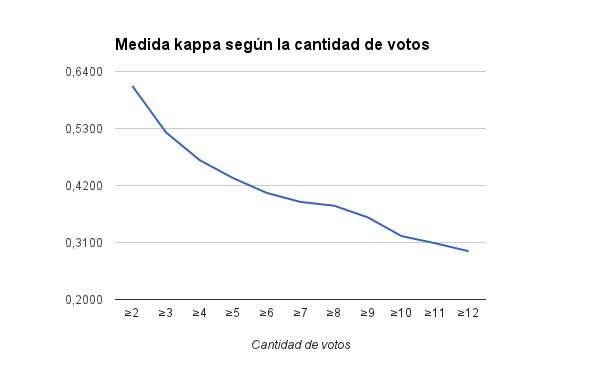
\includegraphics{kappa.png}
    \end{center}

    \note{El resultado obtenido para todos los tweets votados por más de una persona es de 0,6. También calculamos según una cantidad mínima de votos, y vemos que el valor de la medida kappa baja, como lo muestra la gráfica. Esto tiene sentido porque a más cantidad de votantes, más discrepancia posible hay.}

    \framebreak

    \begin{itemize}
        \item \large{0,612; acuerdo de nivel \textbf{medio-alto}}

        \begin{itemize}
            \item No hay unanimidad claramente
        \end{itemize}
    \end{itemize}

    \note{¿Cómo fue el acuerdo entre las personas entonces? Se considera que es bastante bueno, este número es considerado en general bastante bueno. Las personas en general están de acuerdo cuándo un tweet es humor. Aunque notar que es claro que en el humor no hay unanimidad en absoluto, lo cual era esperado.}
\end{frame}
